%% ----------------------------------------------------------------------------
% BIWI SA/MA thesis template
%
% Created 09/29/2006 by Andreas Ess
% Extended 13/02/2009 by Jan Lesniak - jlesniak@vision.ee.ethz.ch
%% ----------------------------------------------------------------------------
\chapter{Related Work}
\label{ch:related_work}
Unsupervised learning has been studied in depth in the past decades. Before the arrival of CNNs handcrafted features like SIFT, HOG and SURF have been solely used for classification and detection~\cite{lee2017}. With deep learning visual representations can be extracted directly from data, but a network often requires millions of labeled images for the supervised learning to produce satisfactory results. In a typical way of working CNNs are trained on large datasets like ImageNet~\cite{deng2009} first and then afterwards fine-tuned to work on a more specific application with limited sources of supervision. 

There are various alternative approaches to circumvent the problem with constructing supervised datasets, learning with an unsupervised approach instead. In reconstruction-based learning a network tries to learn a representation that can reproduce itself, while in self-supervised learning internal context is exploited as supervisory signal.

\section{Reconstruction-based learning}
In a more general sense, we can think of a good image representation as the latent variables of a generative model, but directly inferring this structure is generally intractable~\cite{doersch2015}. One well-researched way to approximate the model is using restricted Boltzmann machines, an generative stochastic artificial neural network trained in various forward and backward passes. A restricted Boltzmann machine contain hidden units that are activated by a stochastic weighted model over the input nodes, and those activations are passed backward in an attempt to reconstruct the input, learning the weights by minimizing reconstruction error~\cite{smolensky1986}. 

Another interesting approach, which works in a similar way, is auto-encoding, where the input image also functions as the output of the network. To build useful features in the hidden layers and thus to prevent learning the identity function, input images are corrupted and the task for the network is to denoise and reconstruct the original image. Often a sparsity penalty is added to allow the technique to be applied in deep networks. It was shown that this approach makes it possible to make robust human body detectors without labeling, but using full-sized images such a network required up to a million CPU hours to learn some valuable representations~\cite{le2013}.  

\section{Self-supervised learning}
Self-supervised learning is another novel unsupervised learning paradigm that exploits different labelings that are freely available besides or within visual data. Those labelings are typically of limited interest for direct estimation outside of some specialized domains. Instead those sources are often processed as a pre-training task with the goal of learning common features that can later be remodeled for other vision tasks such as object detection and semantic segmentation~\cite{misra2016}. 

To achieve this, the networks used by those proposed tasks have a common convolutional backbone pipeline to extract features. Common choices for this multi-layer detection architecture include AlexNet~\cite{krizhevsky2012} (and the closely related CaffeNet~\cite{jia2014}), VGC~\cite{simonyan2014}, GoogleNet~\cite{szegedy2015} and ResNet~\cite{he2016}. To apply the network to, for example, semantic segmentation, the pre-trained architecture are directly integrated into a complete convolutional classification framework, like the state-of-the-art Mask R-CNN~\cite{he2017}, with the weights initialized to those learned using the self-supervised tasks. Finally a labeled dataset of segmented sections, usually of limited size (as labeling is expensive), could then be used to fine-tune the network for classification and segmentation, hoping to achieve better performance.

Recent work has investigated different sources of intrinsic information within image and video data that can be exploited for self-supervision. Most works have focused on the following origins of context: 
\begin{itemize}
\item Spatial structure
\item Spatiotemporal coherence 
\item Auxiliary data, typically in the form of ego-motion.
\end{itemize}
Some examples of these type of tasks are introduced hereafter.

\begin{figure}[t]
\centering
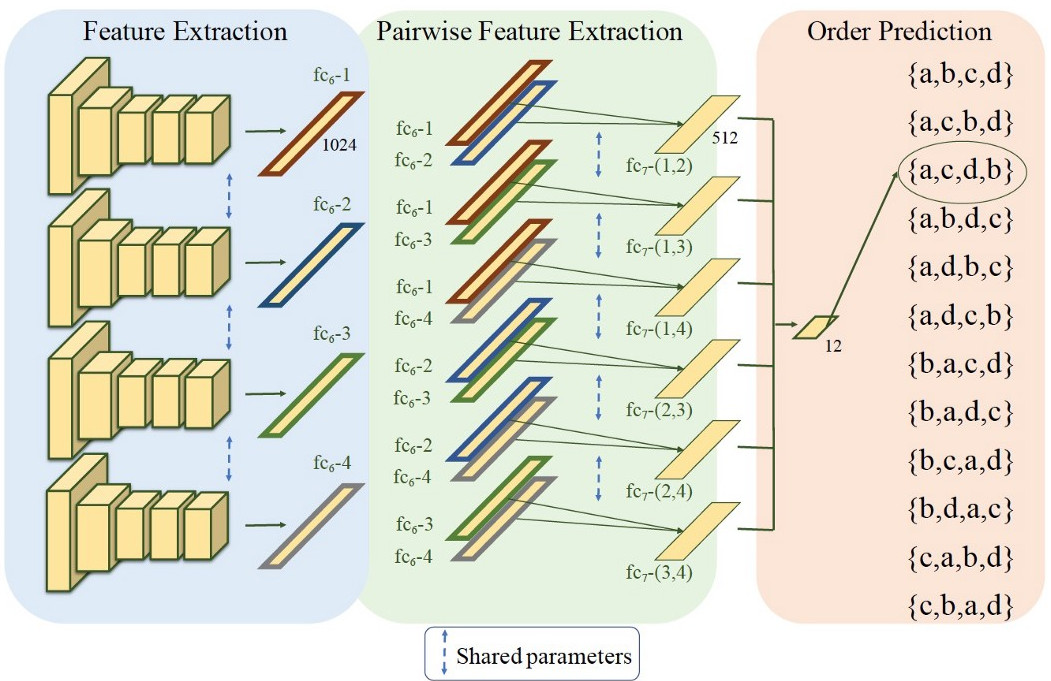
\includegraphics[width=\textwidth]{images/sorting_sequences.jpg}
\caption{Network proposed by Lee et al.\cite{lee2017} to sort a sequence of images. The four shuffled images enter on the right side and the output is a single integer representing a particular permutation. Image is modified from \cite{lee2017}.}
\label{fig:sorting_sequence}
\end{figure}

Doersch et al.~\cite{doersch2015} formulate a self-supervised task to learn spatial context in images. The image is first split in an 3x3 grid, and the patch in the middle of the image is taken together with any of the other 8 tiles. Then the network is trained to learn to predict the correct location of the second tile relative to the first. This work was later extended to observe all the tiles at the same time by shuffling the patches and learning to solve the created jigsaw puzzle~\cite{noroozi2016}, an example which was shown earlier in Figure \ref{fig:jigsaw}. Another related technique was put forward by Wang \& Cupta~\cite{wang2015} that tries to exploit different views of the same object and use known similarity as a training loss. It does this by mining two images of the same object, found using unsupervised KLT-tracking with SURF features in video data, and another unrelated random image. The setup uses a Siamese network for the three images with the final loss penalizing differences in the visual representation of the same object and on the opposite side similarities in comparison with the random image.

This previous approach makes use of temporal coherence, but is ultimately an spatial learning method requiring significant pre-processing to create the similarity task. Misra et al.~\cite{misra2016} opt for an easier way to learn directly from the temporal coherence. They mine sequences of three frames from videos and shuffle these in a random order, using the fact if the permutation is sorted or not as supervision source. This approach was expanded later by Lee et al.~\cite{lee2017} to sequences of longer length with the task of the neural network to learn the full permutation. Their network uses a Caffenet\cite{jia2014} CNN in a Siamese structure for independent feature extraction in the backbone network to a single fully connected layer of 1024 neurons, followed by pair-wise feature extraction between all the fully connected layers that combines into a layer of 512 neurons, and ending in a final fully-connected output layer for the actual order prediction. This network is shown graphically in Figure \ref{fig:sorting_sequence} and will be an important base network for this thesis. In another variation using temporal coherence, a network is fed $N$ correctly ordered tuples and one other in the wrong order. The network can then try to learn to identify the wrongly ordered tuple in all $N+1$ tuple inputs~\cite{fernando2017}. Both approaches makes the learning formulation more complicated, aiming to learn richer representations. 

A final interesting form of supervision is ego-motion, which use the information about movement recorded by additional sensors bound to the vision source. Living species also leverage self-generated movement in concert with visual feedback for proper perceptual development. Inspired by this concept, neural networks should also be able to benefit from information from registered movement. Agrawal et al.~\cite{agrawal2015} directly use information about camera transformations, their agent optimizes its visual representations by minimizing the error between the ego-motion obtained from the motor system and ego-motion predicted using the network only. The two image frames go through a Siamese base architecture followed by fully-connected layers to estimate the transformation. In a similar work Jayaraman \& Grauman~\cite{jayaraman2015} learn a equivariant feature space using ego-motion by mapping the feature space between two frames and calculating the loss based on the difference between the features.

\section{Using 3D lidar data in CNNs}
Earlier work on self-supervision, like most historical work in the field of computer vision, has focused on images, videos and auxiliary signals in the form of ego-motion. This work aims to integrate lidar data to optimize the performance of the network. While lidar data has not been actively applied in the context of self-supervision and historically general focus in object detection has been on RGB images, various earlier works have already investigated the usage of lidar data. Because lidar data is intrinsically 3D, it cannot be handled directly by an 2D neural network. The logical step of adding an extra axis to make the convolutions 3D, will work from a theoretical perspective, but implemented in a naive way will be computationally very expensive, and requires huge amounts of memory. A key finding to optimize the performance is the observation that lidar data is sparse and most of the space is unoccupied~\cite{wang2015vote}, showing possibilities to simplify convolutions significantly by exploiting a duality between sliding window detection with linear classifiers and a voting scheme only from the occupied cells. This approach was later optimized with rectified linear units and a $\lambda_1$ penalty to improve layer sparsity over the entire CNN stack\cite{engelcke2017}. A similar proposal was put forward by Zhou et al.~\cite{zhou2017voxelnet} to combine point-wise features with a locally aggregated feature in the form of a 3D voxel. 

In prior works~\cite{engelcke2017,zhou2017voxelnet,wang2015} using 3D convolutions the focus is on estimating 3D bounding boxes and semantic segmentation, however in our task the lidar data is projected to be used as supplementary signal to boost the learning. As the addition of full 3D data is expected to be relatively marginal, and these approaches remain computationally expensive~\cite{chen2017} an alternative way is to project and discretize the 3D data to 2D front view~\cite{li2016}. This approach can also be extended to a multi-view approach, generating both a bird-eye view and a front-view as has been suggested by Chen et al.~\cite{chen2017}. The usage of 2D projection schemes for lidar data is simpler to combine with image data, as it allows fusing the data from the different networks at different layers of the backbone network. Different fusion schemes have been explored with direct fusion by adding channels to the RGB channel, fusing at early layers and fusing at later layers~\cite{schlosser2016} spitting up the network views in different ways. Deep fusion has been proposed as well by continuously combining and splitting the data at different layers~\cite{chen2017}, but this approach is not researched in more detail in this work.

Before fusing the different layers, a initial question arises how to handle the projected 2D information generated from the lidars. The data projected at different layers will be sparse, leading to many empty cells when discretization is on the same order of magnitude as the image data. For the distances there is no natural way to handle missing data, as the logical initialization value of zero would indicate an object directly in front of the camera, which is often far from correct. Neural networks should technically be able to handle those discrepancies themselves, but additional preprocessing might be beneficial. Dolson et al.~\cite{dolson2010} propose a method to generate an interpolated depth map using a Gaussian interpolation framework in high-dimensional spaces, regularizing the generation of a solution from sparse range data using camera frames to exploit the property that depth discontinuities tend to align in intensity boundaries. An alternative upsampling method by Premebida et al.\cite{premebida2014} generates an dense depth map solely from the sparse range data by simply estimating the depth at a certain pixel as a weighted sum of points from within a certain neighborhood, based on their distance to the pixel and their intensity values (giving higher priority to close detections). This approach gives less sharper boundaries, but is also more rigid to corruption of the depth signal.  

Naturally the lidar data contains information about distances - next to the reflectance values - however it is not directly clear if it best to learn directly from the depth map. Are there transformations of the input that the CNN learns more effectively from? Work by Gupta et al.~\cite{gupta2014} on RGB-D images suggests the use of a so-called HHA encoding, which transforms the depth map into a horizontal disparity map, the height above ground and the angle the pixel's local surface makes with the inferred gravity direction. More details about the construction of these features are given in an earlier work~\cite{gupta2013}. Schossler et al.~\cite{schlosser2016} use this HHA encoding on the depth maps from lidar data generated using the earlier-mentioned weighted upsampling method~\cite{premebida2014} for the purpose of accurate detection of pedestrians.
